\documentclass[11pt,a4paper,oneside]{book}

% ── Essential Packages ──
\usepackage[utf8]{inputenc}
\usepackage[T1]{fontenc}
\usepackage[margin=2.4cm,top=2.6cm,bottom=2.6cm,headheight=26pt]{geometry}

% ── Classic LaTeX Book Typeface ──
\usepackage{lmodern}         % Official Latin Modern Typeface
\usepackage{inconsolata}     % Clean, legible monospaced font for code
\usepackage{microtype}
\usepackage{xcolor}
\usepackage{graphicx}
\usepackage{amsmath,amssymb}
\usepackage{tabularx}
\usepackage{booktabs}
\usepackage{array}
\usepackage{enumitem}
\usepackage{titlesec}
\usepackage{fancyhdr}
\usepackage[most]{tcolorbox}
\usepackage{tikz}
\usetikzlibrary{shapes,arrows,positioning,calc}
\usepackage{listings}
\usepackage{float}

% ── HGG Official Corporate Color Palette ──
\definecolor{HGGNavy}{RGB}{6, 23, 57}         % #061739 - Deep Corporate Navy
\definecolor{HGGBlue}{RGB}{10, 36, 87}        % #0A2457 - Primary Navy
\definecolor{HGGAccentBlue}{RGB}{20, 88, 139} % #14588B - Strategic Blue
\definecolor{HGGCyan}{RGB}{87, 163, 192}      % #57A3C0 - Ice Blue
\definecolor{HGGGold}{RGB}{196, 152, 56}      % #C49838 - Deep Antique Gold
\definecolor{HGGGoldLight}{RGB}{223, 183, 88} % #DFB758 - Bright Champagne Gold
\definecolor{HGGCanvas}{RGB}{248, 250, 252}   % #F8FAFC - Clean Canvas
\definecolor{HGGDarkText}{RGB}{15, 23, 42}    % #0F172A - Body Charcoal
\definecolor{HGGMutedText}{RGB}{100, 116, 139}% #64748B - Muted Text
\definecolor{HGGBorder}{RGB}{226, 232, 240}   % #E2E8F0 - Clean Border
\definecolor{HGGGreen}{RGB}{16, 185, 129}     % #10B981 - Success Green
\definecolor{HGGRed}{RGB}{185, 28, 28}        % #B91C1C - Security Red
\definecolor{HGGSlateLight}{RGB}{241, 245, 249}

% ── Hyperlinks & Metadata ──
\usepackage{hyperref}
\hypersetup{
    colorlinks=true,
    linkcolor=HGGNavy,
    filecolor=HGGGold,
    urlcolor=HGGAccentBlue,
    citecolor=HGGGold,
    plainpages=false,
    pdfpagelabels=true,
    pdftitle={THE HINTER GROUP GHANA LTD — Developer Handover & Production Deployment Manual},
    pdfauthor={Shair Shishir (Lead Technical Consultant)},
    pdfsubject={Technical Deployment, Infrastructure Ownership, DNS, SMTP & CMS Governance},
    pdfkeywords={HGG, Netlify, Next.js, Sanity CMS, Production Deployment, Confidential, Ghana},
    pdfpagemode=UseOutlines,
    bookmarksopen=true
}

% ── Listings Configuration ──
\lstset{
  basicstyle=\footnotesize\ttfamily\color{white},
  backgroundcolor=\color{HGGNavy},
  breaklines=true,
  keepspaces=true,
  columns=flexible,
  frame=single,
  rulecolor=\color{HGGGold},
  framesep=8pt,
  xleftmargin=6pt,
  xrightmargin=6pt,
  showstringspaces=false
}

% ── Chapter & Section Styling (Book Format) ──
\titleformat{\chapter}[display]
  {\normalfont\scshape\color{HGGNavy}}
  {\filright\footnotesize\bfseries\color{HGGGold}CHAPTER \thechapter}
  {0.8ex}
  {\LARGE\bfseries\color{HGGNavy}}
  [\vspace{0.8ex}{\color{HGGGold}\titlerule[1.2pt]}]

\titlespacing*{\chapter}{0pt}{-20pt}{20pt}

\titleformat{\section}
  {\color{HGGNavy}\normalfont\Large\bfseries}
  {\color{HGGGold}\thesection}{0.8em}{}[\color{HGGBorder}\titlerule]

\titleformat{\subsection}
  {\color{HGGNavy}\normalfont\large\bfseries}
  {\color{HGGAccentBlue}\thesubsection}{0.6em}{}

\titleformat{\subsubsection}
  {\color{HGGAccentBlue}\normalfont\normalsize\bfseries}
  {\thesubsubsection}{0.5em}{}

% ── Running Headers & Footers (Clean Single-Sided Layout) ──
\pagestyle{fancy}
\fancyhf{}
\renewcommand{\headrulewidth}{0.5pt}
\renewcommand{\headrule}{\hbox to\headwidth{\color{HGGGold}\leaders\hrule height \headrulewidth\hfill}}
\fancyhead[R]{\small\bfseries\color{HGGNavy}\thepage}
\fancyhead[L]{\small\color{HGGDarkText}\nouppercase{\leftmark}}
\fancyfoot[C]{\footnotesize\color{HGGMutedText}THE HINTER GROUP GHANA LTD $\cdot$ \textbf{\color{HGGRed}STRICTLY CONFIDENTIAL} $\cdot$ REF: \texttt{HGG-MAN-2026-002}}
\renewcommand{\footrulewidth}{0.3pt}
\renewcommand{\footrule}{\hbox to\headwidth{\color{HGGBorder}\leaders\hrule height \footrulewidth\hfill}}

% Redefine plain page style for chapter opening pages
\fancypagestyle{plain}{
  \fancyhf{}
  \fancyfoot[C]{\footnotesize\color{HGGMutedText}THE HINTER GROUP GHANA LTD $\cdot$ \textbf{\color{HGGRed}CONFIDENTIAL} $\cdot$ Page \thepage}
  \renewcommand{\headrulewidth}{0pt}
  \renewcommand{\footrulewidth}{0.3pt}
}

% ── Custom Callout Boxes ──
\newtcolorbox{infobox}[1][]{
  enhanced,
  colback=HGGCanvas,
  colframe=HGGAccentBlue,
  arc=2mm,
  boxrule=1pt,
  left=10pt,
  right=10pt,
  top=6pt,
  bottom=6pt,
  title=\textbf{\color{white}#1},
  coltitle=white,
  colbacktitle=HGGAccentBlue,
  fonttitle=\bfseries\small,
  attach boxed title to top left={yshift=-2mm, xshift=4mm},
  boxed title style={arc=1mm, boxrule=0pt}
}

\newtcolorbox{goldbox}[1][]{
  enhanced,
  colback=HGGCanvas,
  colframe=HGGGold,
  arc=2mm,
  boxrule=1.2pt,
  left=10pt,
  right=10pt,
  top=6pt,
  bottom=6pt,
  title=\textbf{\color{HGGNavy}#1},
  coltitle=HGGNavy,
  colbacktitle=HGGGoldLight,
  fonttitle=\bfseries\small,
  attach boxed title to top left={yshift=-2mm, xshift=4mm},
  boxed title style={arc=1mm, boxrule=0pt}
}

\newtcolorbox{confidentialbox}[1][]{
  enhanced,
  colback=white,
  colframe=HGGRed,
  arc=2mm,
  boxrule=1.2pt,
  left=10pt,
  right=10pt,
  top=6pt,
  bottom=6pt,
  title=\textbf{\color{white}#1},
  coltitle=white,
  colbacktitle=HGGRed,
  fonttitle=\bfseries\small,
  attach boxed title to top left={yshift=-2mm, xshift=4mm},
  boxed title style={arc=1mm, boxrule=0pt}
}

\begin{document}

% ═════════════════════════════════════════════════════════════════
% BOOK COVER PAGE
% ═════════════════════════════════════════════════════════════════
\begin{titlepage}
\pagecolor{white}
\begin{tikzpicture}[remember picture,overlay]
  % Elegant Double Border Frame
  \draw[line width=2.5pt, color=HGGNavy] 
    ($(current page.north west) + (1.2cm,-1.2cm)$) 
    rectangle 
    ($(current page.south east) + (-1.2cm,1.2cm)$);
  \draw[line width=0.8pt, color=HGGGold] 
    ($(current page.north west) + (1.35cm,-1.35cm)$) 
    rectangle 
    ($(current page.south east) + (-1.35cm,1.35cm)$);

  % Corner Ornaments
  \node[anchor=north west, color=HGGGold, xshift=1.5cm, yshift=-1.5cm] at (current page.north west) 
    {\small$\blacklozenge$};
  \node[anchor=north east, color=HGGGold, xshift=-1.5cm, yshift=-1.5cm] at (current page.north east) 
    {\small$\blacklozenge$};
  \node[anchor=south west, color=HGGGold, xshift=1.5cm, yshift=1.5cm] at (current page.south west) 
    {\small$\blacklozenge$};
  \node[anchor=south east, color=HGGGold, xshift=-1.5cm, yshift=1.5cm] at (current page.south east) 
    {\small$\blacklozenge$};
\end{tikzpicture}

\vspace*{0.2cm}

\begin{center}
  % Security Classification Header Badge
  \begin{tcolorbox}[
    width=0.7\textwidth,
    colback=HGGRed!8,
    colframe=HGGRed,
    arc=1.5mm,
    boxrule=1pt,
    center,
    halign=center,
    top=4pt,bottom=4pt
  ]
    \bfseries\color{HGGRed}\small
    $\bigstar$ STRICTLY CONFIDENTIAL // PROPRIETARY DOCUMENT $\bigstar$\\[0.05cm]
    \scriptsize NOT FOR PUBLIC DISSEMINATION $\cdot$ AUTHORIZED PERSONNEL ONLY
  \end{tcolorbox}

  \vspace{0.8cm}

  % Official HGG Emblem Logo
  
\includegraphics[width=4.2cm]{Development/frontend/public/assets/logos/Logo/Logo_Logo.png}

  \vspace{0.6cm}

  {\large\bfseries\color{HGGNavy}THE HINTER GROUP GHANA LTD}\\[0.15cm]
  {\footnotesize\bfseries\color{HGGGold}CONSULTING + VENTURES \ \textbar\ \ BROKERAGE $\cdot$ COMMITTED TO EXCELLENCE}

  \vspace{0.8cm}

  {\color{HGGGold}\rule{0.6\textwidth}{1.5pt}}\\[0.4cm]
  {\fontsize{22}{26}\selectfont\scshape\bfseries\color{HGGNavy} TECHNICAL DEPLOYMENT \&\\[0.2cm] DEVELOPER HANDOVER MANUAL}\\[0.35cm]
  {\large\itshape\color{HGGAccentBlue} An Operational Guide to Continuous Deployment, Monorepo Architecture,\\ DNS Governance, Google SMTP Secrets, and CMS Administration}
  \\[0.4cm]
  {\color{HGGGold}\rule{0.6\textwidth}{1.5pt}}

  \vspace{0.8cm}

  \begin{tcolorbox}[
    width=0.88\textwidth,
    colback=HGGCanvas,
    colframe=HGGBorder,
    arc=2mm,
    boxrule=0.8pt,
    left=14pt,right=14pt,top=8pt,bottom=8pt
  ]
    \centering\footnotesize
    \begin{tabularx}{\linewidth}{rX}
      \textbf{Permanent Target Domain:} & \url{https://hintergroupghana.com} \\
      \textbf{Document Control Number:} & \texttt{HGG-MAN-DEP-2026-002} \\
      \textbf{Security Classification:} & \textbf{\color{HGGRed}CONFIDENTIAL} (Tier-1 Corporate Governance) \\
      \textbf{Technical Handover Lead:} & \textbf{Shair Shishir}, Lead Technical Consultant \& Developer \\
      \textbf{Recipient \& Owner:} & \textbf{Charles N. Hammond}, Founder \& Managing Director \\
      \textbf{Repository Endpoint:} & \url{https://github.com/hintergroupdev/HGG} (\texttt{main}) \\
      \textbf{Publication Date:} & September 2026 (Production Release v2.0) \\
    \end{tabularx}
  \end{tcolorbox}

  \vfill

  {\scriptsize\color{HGGMutedText} \copyright\ 2026 THE HINTER GROUP GHANA LTD. All rights reserved. Registered in Accra, Ghana.}
\end{center}
\end{titlepage}
\nopagecolor

% ═════════════════════════════════════════════════════════════════
% FRONT MATTER: LEGAL & NON-DISCLOSURE
% ═════════════════════════════════════════════════════════════════
\frontmatter
\pagestyle{plain}

\chapter*{Notice of Confidentiality \& Executive Abstract}
\addcontentsline{toc}{chapter}{Notice of Confidentiality \& Executive Abstract}

\begin{confidentialbox}[Confidentiality \& Proprietary Rights Notice]
This technical manual contains proprietary, confidential, and trade-secret information pertaining to the architecture, infrastructure, security tokens, source code, and administrative credentials of \textbf{THE HINTER GROUP GHANA LTD (HGG)}. 

Unauthorized copying, forwarding, electronic transmission, or distribution of this document or any associated credentials without the prior written consent of Charles N. Hammond is strictly prohibited under applicable intellectual property and commercial law.
\end{confidentialbox}

\vspace{0.6cm}

\section*{Abstract}
This technical manual serves as the comprehensive operational handover guide for the official corporate web platform of \textbf{THE HINTER GROUP GHANA LTD (HGG)}, accessible globally at \url{https://hintergroupghana.com}. Authored under a direct corporate infrastructure ownership framework, this document provides complete, step-by-step engineering protocols enabling HGG to govern, deploy, and maintain its digital infrastructure independently without ongoing reliance on third-party developer accounts.

The manual details the end-to-end architecture integrating a high-performance Next.js presentation engine deployed to Netlify's globally distributed Edge Network, coupled with a headless Sanity CMS content repository, Google SMTP mail routing, an enterprise Personnel Identity Verification engine, and native Search Engine Optimization (SEO) with Google Search Console verification. Clear, sequenced operational procedures encompass Git repository linking, monorepo workspace configuration (\texttt{Development/frontend}), production environment secrets injection, Google Workspace application password provisioning, SSL/TLS certificate enforcement, DNS TXT search verification, and comprehensive post-handover validation audits.

\vspace{0.4cm}

\subsection*{Core Engineering Capabilities Handed Over}
\begin{itemize}[leftmargin=1.2cm]
  \item Complete source code, schemas, and assets maintained in the official GitHub repository (\texttt{hintergroupdev/HGG}).
  \item Continuous deployment pipeline connected directly to HGG's native Netlify hosting instance.
  \item Decoupled, serverless contact dispatch infrastructure powered by Google SMTP.
  \item Real-time content administration via Sanity Studio and QR-linked Personnel Verification.
  \item Enterprise on-page SEO generation and Google Search Console DNS TXT verification.
\end{itemize}

\clearpage

% ═════════════════════════════════════════════════════════════════
% TABLE OF CONTENTS
% ═════════════════════════════════════════════════════════════════
\tableofcontents
\clearpage

% ═════════════════════════════════════════════════════════════════
% MAIN MATTER: CHAPTERS
% ═════════════════════════════════════════════════════════════════
\mainmatter
\pagestyle{fancy}

% ─────────────────────────────────────────────────────────────────
% CHAPTER 1
% ─────────────────────────────────────────────────────────────────
\chapter{Executive Architecture \& Handover Strategy}

\section{System Overview}
The official corporate web platform for \textbf{THE HINTER GROUP GHANA LTD (HGG)} has been constructed as an enterprise, high-performance static and serverless application. The architecture decouples the continuous integration and edge hosting infrastructure (Netlify) from the Headless Content Management System (Sanity.io) and corporate mail dispatch services (Google SMTP).

\begin{figure}[h!]
\centering
\resizebox{0.92\textwidth}{!}{%
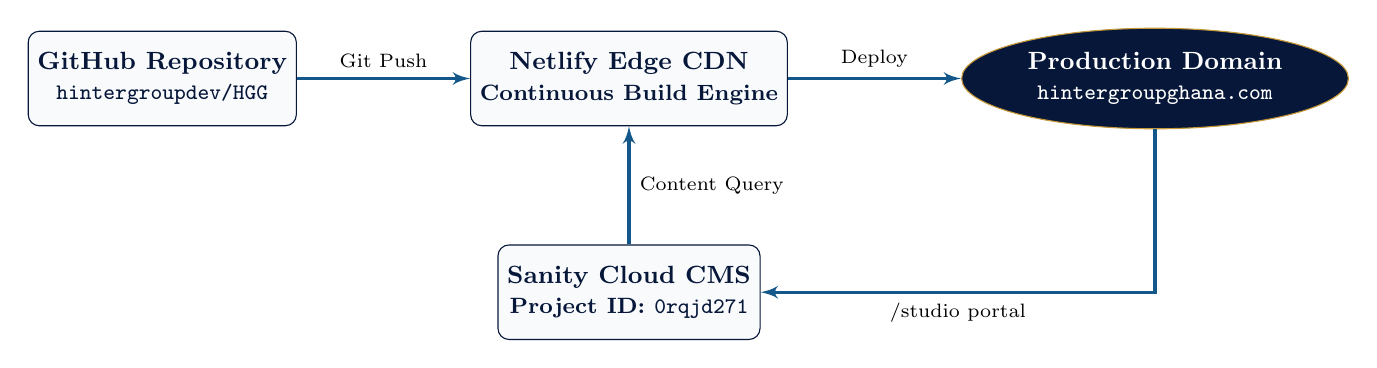
\begin{tikzpicture}[node distance=1.8cm, auto]
  \tikzstyle{block} = [rectangle, draw=HGGNavy, fill=HGGCanvas, text=HGGNavy, rounded corners, minimum height=1.2cm, minimum width=3.2cm, font=\small\bfseries, align=center]
  \tikzstyle{cloud} = [ellipse, draw=HGGGold, fill=HGGNavy, text=white, minimum height=1.2cm, minimum width=3cm, font=\small\bfseries, align=center]
  \tikzstyle{line} = [draw=HGGAccentBlue, -latex', line width=1.2pt]

  \node [block] (git) {GitHub Repository\\\footnotesize\texttt{hintergroupdev/HGG}};
  \node [block, right=2.2cm of git] (netlify) {Netlify Edge CDN\\\footnotesize Continuous Build Engine};
  \node [cloud, right=2.2cm of netlify] (prod) {Production Domain\\\footnotesize\texttt{hintergroupghana.com}};
  \node [block, below=1.5cm of netlify] (sanity) {Sanity Cloud CMS\\\footnotesize Project ID: \texttt{0rqjd271}};

  \path [line] (git) -- node [above] {\scriptsize Git Push} (netlify);
  \path [line] (netlify) -- node [above] {\scriptsize Deploy} (prod);
  \path [line] (sanity) -- node [right] {\scriptsize Content Query} (netlify);
  \path [line] (prod) |- node [near end, below] {\scriptsize /studio portal} (sanity);
\end{tikzpicture}
}
\caption{HGG Enterprise Platform Architecture Diagram}
\label{fig:architecture}
\end{figure}

\section{Direct Infrastructure Ownership Model}
Under direct infrastructure ownership, HGG retains 100\% legal, administrative, and technical control of its production Netlify environment. This eliminates the necessity of purchasing additional third-party team seats while ensuring your organization can independently trigger continuous deployments, rotate security keys, and manage domain records.

% ─────────────────────────────────────────────────────────────────
% CHAPTER 2
% ─────────────────────────────────────────────────────────────────
\chapter{Master Credentials \& Repository Registry}

\section{Master Access Registry}
All code, graphical assets, and deployment templates are preserved in the official repository. Table \ref{tab:credentials} documents the master access parameters.

\begin{table}[H]
\centering
\small
\begin{tabularx}{\textwidth}{lXX}
  \toprule
  \textbf{Resource Item} & \textbf{Identifier / URL} & \textbf{Operational Context} \\
  \midrule
  \textbf{GitHub Repository} & \url{https://github.com/hintergroupdev/HGG} & Complete source code, schemas, and configurations. \\
  \textbf{GitHub Account / Org} & \texttt{hintergroupdev} & Authenticated exclusively via Google Single Sign-On (SSO). \\
  \textbf{Google Master Email} & \texttt{hintergroup.dev@gmail.com} & Master gateway email for GitHub, Netlify, and Sanity. \\
  \textbf{Google Account Password} & \texttt{hintergroup1234} & Master Google account password (gateway credentials). \\
  \textbf{Production Branch} & \texttt{main} & Production-ready branch tracking live releases. \\
  \textbf{Production URL} & \url{https://hintergroupghana.com} & Permanent live website domain. \\
  \textbf{Sanity Studio URL} & \url{https://hintergroupghana.com/studio} & Embedded content management portal. \\
  \textbf{Verification URL} & \url{https://hintergroupghana.com/verify/HGG-001} & Personnel identity verification route. \\
  \bottomrule
\end{tabularx}
\caption{Official Project Credentials and Master Endpoints}
\label{tab:credentials}
\end{table}

\begin{goldbox}[Authentication Architecture: Google Single Sign-On (SSO)]
\textbf{Crucial Note on Credentials:} \texttt{hintergroupdev} and \texttt{hintergroup1234} are \textbf{not} standalone GitHub username and password credentials. GitHub does not have a native password for this account.
\begin{itemize}[leftmargin=*]
  \item In all portals (GitHub, Netlify, Sanity Studio), access is authenticated by selecting \textbf{``Sign in with GitHub''}.
  \item Whenever no active GitHub session exists, GitHub requires selecting \textbf{``Sign in with Google''} using \textbf{\texttt{hintergroup.dev@gmail.com}} and password \textbf{\texttt{hintergroup1234}}.
\end{itemize}
\end{goldbox}

\section{Initial Login \& Repository Access Protocol}
Before linking Netlify or modifying environment variables, the client administration should authenticate into the official accounts in the following required sequence:

\begin{enumerate}[leftmargin=*,label=\textbf{Step \arabic*:}]
  \item \textbf{Log In to the Project Email First:}
    Open a web browser and navigate to Google / Gmail:
    \begin{center}
      \url{https://mail.google.com}
    \end{center}
    Sign in with the project developer account:
    \begin{itemize}[leftmargin=1.2cm]
      \item \textbf{Email Address:} \texttt{hintergroup.dev@gmail.com}
      \item \textbf{Google Password:} \texttt{hintergroup1234}
    \end{itemize}
    \textit{Operational Note: Keep this Gmail inbox open in your browser tab. When signing in to GitHub from a new computer, IP address, or location, security verification codes will arrive here.}

  \item \textbf{Sign In to GitHub via Google SSO:}
    In a new browser tab, navigate to the GitHub authentication portal:
    \begin{center}
      \url{https://github.com/login}
    \end{center}
    \textbf{Important:} Do not enter \texttt{hintergroupdev} or \texttt{hintergroup1234} into GitHub's native login fields. The account has no independent GitHub password and is connected via Google Single Sign-On (SSO). Follow these steps:
    \begin{itemize}[leftmargin=1.2cm]
      \item Click \textbf{Sign in with Google} (or \textit{Continue with Google}).
      \item On the Google account selection screen, select the active project account:\\
        \textbf{\texttt{hintergroup.dev@gmail.com}} (already signed in from Step 1).
      \item GitHub will verify the Google session and grant access to \textbf{\texttt{hintergroupdev}}.
      \item If GitHub displays a one-time device verification screen, switch to the open Gmail tab, copy the 6-digit code received from GitHub, and enter it to complete sign-in.
    \end{itemize}

  \item \textbf{Navigate Directly to the Master Repository:}
    Once successfully authenticated, visit the HGG production repository:
    \begin{center}
      \Large\bfseries\url{https://github.com/hintergroupdev/HGG}
    \end{center}
    Confirm that the active branch is set to \textbf{\texttt{main}} and verify that you possess full administrative ownership over the codebase.
\end{enumerate}

\begin{goldbox}[Password Hygiene Recommendation]
Following successful production deployment, it is advised to log into \url{https://github.com} and \url{https://myaccount.google.com} as \texttt{hintergroup.dev@gmail.com} to update account passwords to your internal corporate standard.
\end{goldbox}

\section{Repository Monorepo Layout}
The repository utilizes a modular structure where the production website application resides in the dedicated workspace directory \texttt{Development/frontend}:

\begin{lstlisting}
HGG/                             <-- Repository Root
+-- netlify.toml                 <-- Root build & security headers
+-- Development/
    \-- frontend/                <-- CRITICAL: NEXT.JS APP ROOT
        +-- app/                 <-- App Router (Pages, Verification, Studio)
        |   +-- page.js          <-- Homepage
        |   +-- about-us/        <-- About Us (Foundation & Focus Areas)
        |   +-- expertise/       <-- Service Pillars & Disciplines
        |   +-- leadership/      <-- Executive Profiles
        |   +-- verify/[id]/     <-- Personnel ID Verification & QR
        |   +-- studio/          <-- Sanity CMS Web Portal
        |   \-- api/contact/     <-- SMTP Contact Form Dispatcher
        +-- components/          <-- Reusable UI, Navbars, Footers
        +-- sanity/              <-- CMS Schemas & Data Queries
        +-- public/assets/       <-- Vector Logos, Favicons, QR Art
        +-- package.json         <-- Node.js Dependencies & Scripts
        \-- netlify.toml         <-- App-level Security & Routing
\end{lstlisting}

% ─────────────────────────────────────────────────────────────────
% CHAPTER 3
% ─────────────────────────────────────────────────────────────────
\chapter{Netlify Re-Linking Protocol}

\section{Preserving the Existing Project \& Domain}
Because HGG already possesses an active Netlify site with \texttt{hintergroupghana.com} configured, \textbf{do not delete the project or create a new site}. Re-linking the repository directly inside the existing project preserves your custom domain, Let's Encrypt SSL certificates, and DNS records.

\section{Step-by-Step Re-linking Sequence}

Follow these 4 brief steps inside your Netlify dashboard:

\begin{enumerate}[leftmargin=*,label=\textbf{Step \arabic*:}]
  \item \textbf{Open Your Active Site in Netlify:}
    Sign in at \url{https://app.netlify.com} (select \textbf{Log in with GitHub}; with your active browser session from Chapter 2, Netlify authenticates automatically), go to the \textbf{Sites} tab, and click on your active production site (\url{https://hintergroupghana.com}).

  \item \textbf{Navigate to Continuous Deployment:}
    In the left sidebar, click \textbf{Site configuration} $\rightarrow$ select \textbf{Build \& deploy} $\rightarrow$ open \textbf{Continuous deployment}.

  \item \textbf{Connect to GitHub:}
    In the \textbf{Repository} settings card:
    \begin{itemize}[leftmargin=1.2cm]
      \item If an older repository is currently attached: Click \textbf{Manage repository} $\rightarrow$ select \textbf{Link to a different repository} (or \textbf{Unlink repository}).
      \item If no repository is linked: Click \textbf{Link repository}.
      \item In the Git provider modal, choose \textbf{GitHub}.
    \end{itemize}

  \item \textbf{Authorize \& Select Repository:}
    When the GitHub authorization window appears:
    \begin{itemize}[leftmargin=1.2cm]
      \item Authorize Netlify under the \texttt{hintergroupdev} account (or select organization \texttt{hintergroupdev}).
      \item Search and select the master repository: \textbf{\texttt{hintergroupdev/HGG}}.
      \item Ensure the deployment branch is set to \textbf{\texttt{main}}.
      \item Click the primary \textbf{Deploy site} (or \textbf{Deploy} / \textbf{Save}) button to confirm the repository connection.
    \end{itemize}
\end{enumerate}

% ─────────────────────────────────────────────────────────────────
% CHAPTER 4
% ─────────────────────────────────────────────────────────────────
\chapter{Build Settings Specification}

\section{Mandatory Monorepo Paths}
In your Netlify dashboard, navigate to \textbf{Site configuration} $\rightarrow$ \textbf{Build \& deploy} $\rightarrow$ \textbf{Continuous deployment}, locate the \textbf{Build settings} section, click \textbf{Edit settings}, and enter the following values:

\begin{table}[h!]
\centering
\small
\begin{tabularx}{\textwidth}{lXX}
  \toprule
  \textbf{Setting Field} & \textbf{Exact Value to Enter} & \textbf{Operational Context} \\
  \midrule
  \textbf{Base directory} & \texttt{Development/frontend} & Directs Netlify into the Next.js application workspace. \\
  \textbf{Build command} & \texttt{npm run build} & Compiles optimized SSR bundles and pages. \\
  \textbf{Publish directory} & \texttt{.next} & Build artifact directory (relative to Base directory). \\
  \textbf{Branch to deploy} & \texttt{main} & Master branch tracking stable production releases. \\
  \bottomrule
\end{tabularx}
\caption{Required Netlify Build Configuration Fields}
\label{tab:build-params}
\end{table}

\begin{infobox}[Notice on Publish Directory]
Because the \textbf{Base directory} is already set to \texttt{Development/frontend}, Netlify automatically resolves all paths from inside that subfolder. Enter \textbf{\texttt{.next}} only as the Publish directory. Do not write \texttt{Development/frontend/.next}.
\end{infobox}

\vspace{0.2cm}

\begin{goldbox}[Action: Triggering the Deployment]
Once the parameters above are entered, click the primary \textbf{Deploy site} (or \textbf{Deploy} / \textbf{Save}) button at the bottom of the settings card to trigger the continuous build process.
\end{goldbox}

% ─────────────────────────────────────────────────────────────────
% CHAPTER 5
% ─────────────────────────────────────────────────────────────────
\chapter{Environment Variables \& Secrets (.env)}

\section{Configuration Block \& Mandatory Modifications}
In Netlify, navigate to \textbf{Site configuration} $\rightarrow$ \textbf{Environment variables}, click \textbf{Add a variable} $\rightarrow$ select \textbf{Import from a .env file}, and paste the block below.

\begin{confidentialbox}[Critical Instruction: Modify Placeholders Before Saving]
\textbf{Do NOT save with raw placeholder values.} You may paste the configuration block below, but you \textbf{must modify the 3 email credential values} before clicking Save:
\begin{itemize}[leftmargin=1.0cm,noitemsep,topsep=1pt]
  \item \textbf{\texttt{SMTP\_USER}:} Replace with your sender Google email (\texttt{hintergroup.dev@gmail.com}).
  \item \textbf{\texttt{SMTP\_PASS}:} Replace with the 16-character Google App Password (Chapter 6).
  \item \textbf{\texttt{CONTACT\_RECEIVER\_EMAIL}:} Replace with your corporate receiving inbox.
\end{itemize}
\end{confidentialbox}

\vspace{-0.15cm}
\begin{lstlisting}[basicstyle=\scriptsize\ttfamily\color{white},framesep=5pt]
NEXT_PUBLIC_SITE_URL=https://hintergroupghana.com
NEXT_PUBLIC_SANITY_PROJECT_ID=0rqjd271
NEXT_PUBLIC_SANITY_DATASET=production
NEXT_PUBLIC_SANITY_API_VERSION=2024-08-30
SANITY_API_READ_TOKEN=
SMTP_HOST=smtp.gmail.com
SMTP_PORT=465
SMTP_SECURE=true
SMTP_USER=YOUR_SENDER_GMAIL_HERE
SMTP_PASS=YOUR_16_DIGIT_APP_PASSWORD_HERE
CONTACT_RECEIVER_EMAIL=YOUR_RECEIVING_INBOX_HERE
\end{lstlisting}

\vspace{-0.1cm}
\section{Parameter Explanations}
\vspace{-0.1cm}

\begin{table}[H]
\centering
\footnotesize
\renewcommand{\arraystretch}{1.08}
\begin{tabularx}{\textwidth}{lXX}
  \toprule
  \textbf{Variable Key} & \textbf{Value / Source} & \textbf{Operational Role} \\
  \midrule
  \texttt{NEXT\_PUBLIC\_SITE\_URL} & \texttt{https://hintergroupghana.com} & Canonical URL for SEO and QR verification. \\
  \texttt{NEXT\_PUBLIC\_SANITY\_PROJECT\_ID} & \texttt{0rqjd271} & HGG's Sanity database identifier. \\
  \texttt{NEXT\_PUBLIC\_SANITY\_DATASET} & \texttt{production} & Primary live data store. \\
  \texttt{NEXT\_PUBLIC\_SANITY\_API\_VERSION} & \texttt{2024-08-30} & Fixed API version lock. \\
  \texttt{SANITY\_API\_READ\_TOKEN} & \textit{(Leave Empty)} & Public read permissions enabled; token not required. \\
  \texttt{SMTP\_HOST} & \texttt{smtp.gmail.com} & Google SMTP server for contact form dispatch. \\
  \texttt{SMTP\_PORT} & \texttt{465} & Secure SSL port. \\
  \texttt{SMTP\_SECURE} & \texttt{true} & Enforces SSL socket encryption. \\
  \texttt{SMTP\_USER} & \textit{Sender Google Address} & Email address utilized to transmit contact notifications. \\
  \texttt{SMTP\_PASS} & \textit{16-Digit App Password} & Dedicated Google Application Password (Chapter 6). \\
  \texttt{CONTACT\_RECEIVER\_EMAIL} & \textit{Recipient Inbox} & Destination corporate inbox (e.g. \texttt{info@...}). \\
  \bottomrule
\end{tabularx}
\caption{Environment Variables Specification}
\label{tab:env-vars}
\end{table}

% ─────────────────────────────────────────────────────────────────
% CHAPTER 6
% ─────────────────────────────────────────────────────────────────
\chapter{Google SMTP \& App Password Setup}

\section{Security Rationale}
To protect corporate accounts against credential stuffing and brute-force intrusion, Google prohibits automated web servers from authenticating using primary account passwords. Instead, Google requires a \textbf{16-character dedicated Application Password}.

\begin{goldbox}[Prerequisite]
Google requires \textbf{2-Step Verification} to be active on the sending account before an Application Password can be generated.
\end{goldbox}

\section{Step-by-Step Generation Protocol}

\begin{enumerate}[leftmargin=*,label=\textbf{Step \arabic*:}]
  \item \textbf{Access Account Security:}
    Log into the Google/Gmail account you designated for \texttt{SMTP\_USER} (such as \texttt{hintergroup.dev@gmail.com} or your corporate Google Workspace address) and visit:
    \begin{center}
      \url{https://myaccount.google.com/security}
    \end{center}

  \item \textbf{Verify 2-Step Verification Status:}
    Under the \textit{"How you sign in to Google"} section, ensure \textbf{2-Step Verification} is set to \textbf{On}. If not, complete the prompt using your mobile device.

  \item \textbf{Generate the 16-Character Password:}
    \begin{itemize}[leftmargin=1.5cm]
      \item In the search box at the top of the Google Account portal, type: \textbf{\texttt{App passwords}} and select it.
      \item In the \textbf{App name} field, enter: \texttt{HGG Website Contact Form}.
      \item Click \textbf{Create}.
      \item Google will display a popup containing a \textbf{16-character code} (formatted like \texttt{xxxx xxxx xxxx xxxx}).
      \item Copy this 16-character string immediately.
    \end{itemize}

  \item \textbf{Save in Netlify:}
    \begin{itemize}[leftmargin=1.5cm]
      \item Return to Netlify $\rightarrow$ \textbf{Site configuration} $\rightarrow$ \textbf{Environment variables}.
      \item Set \texttt{SMTP\_PASS} to your 16-character code.
      \item Set \texttt{SMTP\_USER} to your Google address.
      \item Set \texttt{CONTACT\_RECEIVER\_EMAIL} to your corporate inquiry inbox.
      \item Click \textbf{Save}.
    \end{itemize}
\end{enumerate}

% ─────────────────────────────────────────────────────────────────
% CHAPTER 7
% ─────────────────────────────────────────────────────────────────
\chapter{Production Deployment \& SSL Verification}

\section{Triggering the Deploy}
With the repository linked and secrets configured, you can launch the live build:
\begin{enumerate}
  \item In the Netlify dashboard, click the \textbf{Deploys} tab in the top navigation.
  \item Click \textbf{Trigger deploy} $\rightarrow$ select \textbf{Deploy site} (or \textbf{Clear cache and deploy site}).
  \item Click on the active deploy to view the streaming build terminal.
  \item The build sequence will complete within 2 minutes with:
    \begin{center}
      \bfseries\color{HGGGreen}Site deploy was successfully published!
    \end{center}
\end{enumerate}

\section{Domain \& SSL Health Check}
\begin{enumerate}
  \item Go to \textbf{Site configuration} $\rightarrow$ \textbf{Domain management}.
  \item Verify that \texttt{hintergroupghana.com} displays with a green checkmark as the \textbf{Primary domain}.
  \item Scroll to \textbf{HTTPS}: verify that an active \textbf{Let's Encrypt SSL certificate} is issued. If not, click \textbf{Verify DNS configuration} $\rightarrow$ \textbf{Provision certificate}.
\end{enumerate}

% ─────────────────────────────────────────────────────────────────
% CHAPTER 8
% ─────────────────────────────────────────────────────────────────
\chapter{Sanity Studio CMS Administration}
\label{chap:sanity}

\section{Accessing the Live CMS Portal}
The Content Management Studio is embedded natively within the production website:
\begin{center}
  \Large\bfseries\url{https://hintergroupghana.com/studio}
\end{center}

\section{Signing In to Sanity Studio}
Sanity Studio authentication is federated through GitHub. Follow these exact steps:
\begin{enumerate}[leftmargin=*,label=\textbf{\arabic*.}]
  \item On the Sanity Studio login screen, click \textbf{Sign in with GitHub}.
  \item \textbf{If you already have an active GitHub session} in your browser (from Chapter 2):\\
    Sanity Studio will immediately authenticate and grant you access to the HGG Content Studio dashboard.
  \item \textbf{If no active GitHub session exists (e.g., in a private or new browser window):}
    \begin{itemize}[leftmargin=1.2cm]
      \item The GitHub login portal will appear.
      \item \textbf{Do NOT attempt to type \texttt{hintergroupdev} or \texttt{hintergroup1234} into the GitHub username/password fields} (they are not standalone GitHub credentials).
      \item Click \textbf{Sign in with Google} (or \textit{Continue with Google}).
      \item Choose or enter \textbf{\texttt{hintergroup.dev@gmail.com}} and password \textbf{\texttt{hintergroup1234}}.
      \item If prompted, click \textbf{Authorize Sanity.io}.
    \end{itemize}
  \item You will enter the HGG Content Studio with full administrator privileges.
\end{enumerate}

\section{Inviting Colleagues \& Assigning Editorial Roles}
To grant access to executives or HR staff using their personal or corporate emails without sharing GitHub credentials:
\begin{enumerate}[leftmargin=*,label=\textbf{\arabic*.}]
  \item Visit the Sanity Management Console: \url{https://www.sanity.io/manage}.
  \item Click \textbf{Log in with GitHub}. (If GitHub prompts for login, select \textbf{Sign in with Google} using \texttt{hintergroup.dev@gmail.com}).
  \item Select project \textbf{HGG} (Project ID: \texttt{0rqjd271}).
  \item Click the \textbf{Members} tab in the top navigation bar.
  \item Click \textbf{Invite Member}.
  \item Enter the colleague's email address and assign an appropriate role:
    \begin{itemize}
      \item \textbf{Administrator:} Complete control over schema, dataset, user permissions, and billing.
      \item \textbf{Editor:} Permission to update site text, post articles, and issue employee credentials.
    \end{itemize}
  \item Click \textbf{Send Invite}. The recipient will receive an activation email and can subsequently log in directly at \url{https://hintergroupghana.com/studio}.
\end{enumerate}

% ─────────────────────────────────────────────────────────────────
% CHAPTER 9
% ─────────────────────────────────────────────────────────────────
\chapter{Search Engine Optimization \& Google Search Console}
\label{chap:seo}

\section{Native Enterprise SEO Architecture}
The HGG corporate web platform incorporates automated, enterprise-grade search engine optimization natively within the application code. Every page is pre-rendered with complete metadata, semantic markup, and crawler assets:

\begin{itemize}[leftmargin=1.2cm]
  \item \textbf{Dynamic Metadata Engine (\texttt{app/layout.js}):} Employs the Next.js Metadata API to dynamically construct page titles using the corporate format (\texttt{\%s | HGG}), tailored meta descriptions, targeted keywords, author and publisher attribution, and canonical link tags enforcing \url{https://hintergroupghana.com} to prevent duplicate indexing.
  \item \textbf{Social Graph Previews (OpenGraph \& Twitter Cards):} Full OpenGraph (\texttt{og:title}, \texttt{og:description}, \texttt{og:image}, \texttt{og:url}) and Twitter Card metadata (\texttt{summary\_large\_image}) are generated automatically. High-resolution $1200\times630$px preview cards display seamlessly whenever links are shared on LinkedIn, WhatsApp, X, or corporate messengers.
  \item \textbf{Structured Data (Schema.org JSON-LD):} Injected via \texttt{components/seo/JsonLd.jsx} across every page, defining HGG as an official \texttt{Corporation} / \texttt{Organization} entity. Microdata fields register legal entity naming, official logo endpoints, headquarters location (Accra, Ghana), contact points, and verified URLs to qualify HGG for Google Knowledge Graph recognition.
  \item \textbf{Automated XML Sitemap (\texttt{sitemap.xml}):}\\
    Programmed dynamically in \texttt{app/sitemap.js} and accessible at \url{https://hintergroupghana.com/sitemap.xml}. Automatically indexes all static marketing routes alongside every dynamic Insights article published via Sanity CMS, assigning respective \texttt{lastModified} timestamps, \texttt{changeFrequency}, and crawl \texttt{priority} weights.
  \item \textbf{Search Engine Crawl Directives (\texttt{robots.txt}):}\\
    Configured in \texttt{app/robots.js} and accessible at \url{https://hintergroupghana.com/robots.txt}. Provides explicit crawl directives for Googlebot, Bingbot, and Applebot. Allows public indexing of corporate content while securely disallowing internal administrative routes (\texttt{/studio/}, \texttt{/api/}, \texttt{/verify/}), and directly references the live XML sitemap.
  \item \textbf{Web App Manifest (\texttt{app/manifest.js}):} Provides Progressive Web App (PWA) manifest compliance, enabling mobile browsers to index standalone app capabilities and icons.
\end{itemize}

\section{The Strategic Purpose of Google Search Console}
While the codebase automatically generates all technical SEO signals, search engines require formal domain ownership verification to activate search indexing. Google Search Console (GSC) is Google's official webmaster platform, serving critical operational functions:
\begin{enumerate}[leftmargin=1.2cm]
  \item \textbf{Search Indexing Activation:} Explicitly informs Googlebot of the live domain, initiating scheduled indexing across worldwide Google Search results.
  \item \textbf{Direct Sitemap Ingestion:} Directly ingests \texttt{sitemap.xml} so new corporate pages and Sanity CMS news publications are indexed rapidly.
  \item \textbf{Search Performance Analytics:} Tracks organic impressions, search queries, click-through rates (CTR), and average ranking positions for HGG brand keywords.
  \item \textbf{Health \& Security Monitoring:} Automatically alerts the organization to broken links, mobile usability faults, Core Web Vitals performance, and security notifications.
\end{enumerate}

\section{DNS TXT Verification Protocol}
Google provides several verification mechanisms. The \textbf{DNS TXT Record method via the Domain property} is the industry standard and the required method for HGG, as it universally verifies all subdomains (\texttt{hintergroupghana.com} and \texttt{www.hintergroupghana.com}) and all protocols (\texttt{http} and \texttt{https}) simultaneously.

\begin{enumerate}[leftmargin=*,label=\textbf{Step \arabic*:}]
  \item \textbf{Access Google Search Console:}
    Open a web browser and navigate to the Google Search Console portal:
    \begin{center}
      \url{https://search.google.com/search-console}
    \end{center}
    Sign in using the master corporate Google account:\\
    \textbf{\texttt{hintergroup.dev@gmail.com}}.

  \item \textbf{Select the Domain Property Type:}
    On the \textbf{Select property type} modal screen:
    \begin{itemize}[leftmargin=1.2cm]
      \item Choose the \textbf{Domain} option (left card), \textit{not} the ``URL prefix'' card.
      \item Enter the root domain name exactly without prefixes or slashes:
        \begin{center}
          \Large\bfseries\texttt{hintergroupghana.com}
        \end{center}
      \item Click \textbf{Continue}.
    \end{itemize}

  \item \textbf{Copy the Unique DNS TXT Verification String:}
    Google will open a dialog window entitled \textbf{Verify domain ownership via DNS record}:
    \begin{itemize}[leftmargin=1.2cm]
      \item In the \textbf{Record type} dropdown, ensure \textbf{TXT} is selected (recommended).
      \item Google displays a unique verification key formatted as:
        \begin{center}
          \small\texttt{google-site-verification=XXXXXXXXXXXXXXXXXXXXXXXXXXXXXXXXXXXXXXXXXXX}
        \end{center}
      \item Click the \textbf{Copy} button to save this complete string to your clipboard.
    \end{itemize}

  \item \textbf{Add the TXT Record to Your DNS Provider:}
    Log in to the DNS provider dashboard managing the nameservers for \texttt{hintergroupghana.com} (e.g., Netlify DNS, Cloudflare, Namecheap, or your corporate domain registrar).
    \begin{itemize}[leftmargin=1.2cm]
      \item Navigate to \textbf{DNS Management} (or \textbf{DNS Settings / Zone Editor}).
      \item Click \textbf{Add new record} (or \textit{Add record}).
      \item Configure the new record parameters as specified in Table \ref{tab:dns_gsc}:
    \end{itemize}

    \begin{table}[H]
    \centering
    \small
    \begin{tabularx}{\textwidth}{llX}
      \toprule
      \textbf{DNS Record Field} & \textbf{Value to Enter} & \textbf{Operational Purpose} \\
      \midrule
      \textbf{Record Type} & \texttt{TXT} & Text verification record. \\
      \textbf{Name / Host} & \texttt{@} (or \texttt{hintergroupghana.com}) & Root apex domain pointer. \\
      \textbf{Value / Content} & \textit{Paste Google TXT string} & \texttt{google-site-verification=...} \\
      \textbf{TTL} & \texttt{3600} (or \texttt{1 hour} / \texttt{Auto}) & Time-To-Live DNS cache duration. \\
      \bottomrule
    \end{tabularx}
    \caption{DNS TXT Record Configuration for Google Search Console}
    \label{tab:dns_gsc}
    \end{table}

    \begin{itemize}[leftmargin=1.2cm]
      \item Click \textbf{Save} (or \textit{Create Record}).
    \end{itemize}

  \item \textbf{Confirm Verification in Google Search Console:}
    Return to the open Google Search Console browser tab and click the green \textbf{Verify} button.
    \begin{itemize}[leftmargin=1.2cm]
      \item \textit{Propagation Note:} DNS updates typically propagate across global recursive resolvers within 2 to 15 minutes. If Google initially reports that the verification token was not found, wait 5 minutes and click \textbf{Verify} again.
      \item When verification succeeds, Google will display a confirmation dialog: \textbf{Ownership verified}.
      \item Click \textbf{Go to property} to open your new domain dashboard.
    \end{itemize}

  \item \textbf{Submit the Production XML Sitemap:}
    To initiate immediate web crawler indexing:
    \begin{itemize}[leftmargin=1.2cm]
      \item In the left-hand navigation sidebar, click \textbf{Sitemaps} (under the \textbf{Indexing} group).
      \item In the \textbf{Add a new sitemap} text box, enter:
        \begin{center}
          \Large\bfseries\texttt{sitemap.xml}
        \end{center}
        (\textit{Note:} The domain prefix \url{https://hintergroupghana.com/} is automatically prepended by Google).
      \item Click \textbf{Submit}.
      \item Google Search Console will process the request and update the status column to \textbf{Success}. Googlebot will now continuously ingest and refresh all website pages and CMS publications.
    \end{itemize}
\end{enumerate}

% ─────────────────────────────────────────────────────────────────
% CHAPTER 10
% ─────────────────────────────────────────────────────────────────
\chapter{Quality Assurance \& Verification Protocols}
\label{chap:qa}

Following deployment, execute the following five validation checks:
\begin{enumerate}[leftmargin=*,label=\textbf{\arabic*.}]
  \item \textbf{Personnel Verification System \& QR Audit:}
    \begin{itemize}
      \item Open: \url{https://hintergroupghana.com/verify/HGG-001}
      \item Verify the green shield badge displays \textbf{IDENTITY VERIFIED}.
      \item Verify the live clock is active and synchronized to \textbf{Accra, Ghana (GMT)} time.
      \item Verify that strictly public professional credentials appear (Photo, Name, Title, Org, Status, Issue Date).
      \item Verify that \textbf{no confidential HR data} (DOB, home address, personal phone/email, national ID) appears on the page.
      \item Scan the physical QR code on the sample ID card using a smartphone camera (iOS / Android); it must open directly to \url{https://hintergroupghana.com/verify/HGG-001}.
    \end{itemize}

  \item \textbf{Contact Desk Email Routing Test:}
    \begin{itemize}
      \item Open: \url{https://hintergroupghana.com/contact}
      \item Submit a test inquiry with your name and email.
      \item Check the inbox defined in \texttt{CONTACT\_RECEIVER\_EMAIL} to verify prompt delivery.
    \end{itemize}

  \item \textbf{CMS Live Synchronization Test:}
    \begin{itemize}
      \item Log into \url{https://hintergroupghana.com/studio}.
      \item Make a minor test edit (e.g. updating office phone or an article excerpt) and click \textbf{Publish}.
      \item Refresh the public site to confirm the update reflects immediately.
    \end{itemize}

  \item \textbf{Multi-Device Responsive Audit:}
    \begin{itemize}
      \item Verify layout on Desktop (Chrome, Safari, Edge).
      \item Verify layout on Tablet (iPad, Android Tablet).
      \item Verify layout on Mobile (iPhone iOS, Android).
      \item Ensure mobile hamburger navigation opens smoothly and no horizontal scroll occurs.
    \end{itemize}

  \item \textbf{Search Engine Optimization \& Sitemap Audit:}
    \begin{itemize}
      \item Open: \url{https://hintergroupghana.com/sitemap.xml} in your browser; verify that all corporate routes and insights articles render cleanly in valid XML.
      \item Open: \url{https://hintergroupghana.com/robots.txt}; verify that search engine crawlers (Googlebot, Bingbot, Applebot) are granted access, while administrative routes are protected.
      \item Check Google Search Console to confirm the Domain property displays verified status and the sitemap reports \textbf{Success}.
    \end{itemize}
\end{enumerate}

% ─────────────────────────────────────────────────────────────────
% CHAPTER 11
% ─────────────────────────────────────────────────────────────────
\chapter{Operational Continuity \& Support SLA}
\label{chap:support}

\section{Automated Git Workflow}
Any future code updates, design enhancements, or schema additions pushed to the \texttt{main} branch of \url{https://github.com/hintergroupdev/HGG} will automatically trigger a Netlify production build. Zero manual intervention is required.

\section{Technical Support Protocol}
If you or your team experience any difficulty during this deployment:
\begin{enumerate}
  \item Note the specific chapter and step number where the issue arose.
  \item Capture a screenshot of the Netlify build terminal or error dialog.
  \item Contact me directly, and I will assist you until the deployment is completed.
\end{enumerate}

\vfill

\begin{center}
  {\color{HGGGold}\rule{0.6\textwidth}{1.2pt}}\\[0.3cm]
  \small\bfseries\color{HGGNavy}THE HINTER GROUP GHANA LTD $\cdot$ COMMITTED TO EXCELLENCE\\[0.1cm]
  \footnotesize\color{HGGMutedText}Accra, Ghana $\cdot$ West Africa $\cdot$ \url{https://hintergroupghana.com}\\[0.3cm]
  {\color{HGGGold}\rule{0.6\textwidth}{1.2pt}}
\end{center}

\end{document}
